	\par The modules themselves will be constructed on 6x8 cm perf-board and will be contained in a housing. Each module will contain all circuitry necessary including power, data acquisition and transmission. 
	\begin{figure}[h!]
		\centering
		\begin{subfigure}[t]{0.45\textwidth}
			\centering
			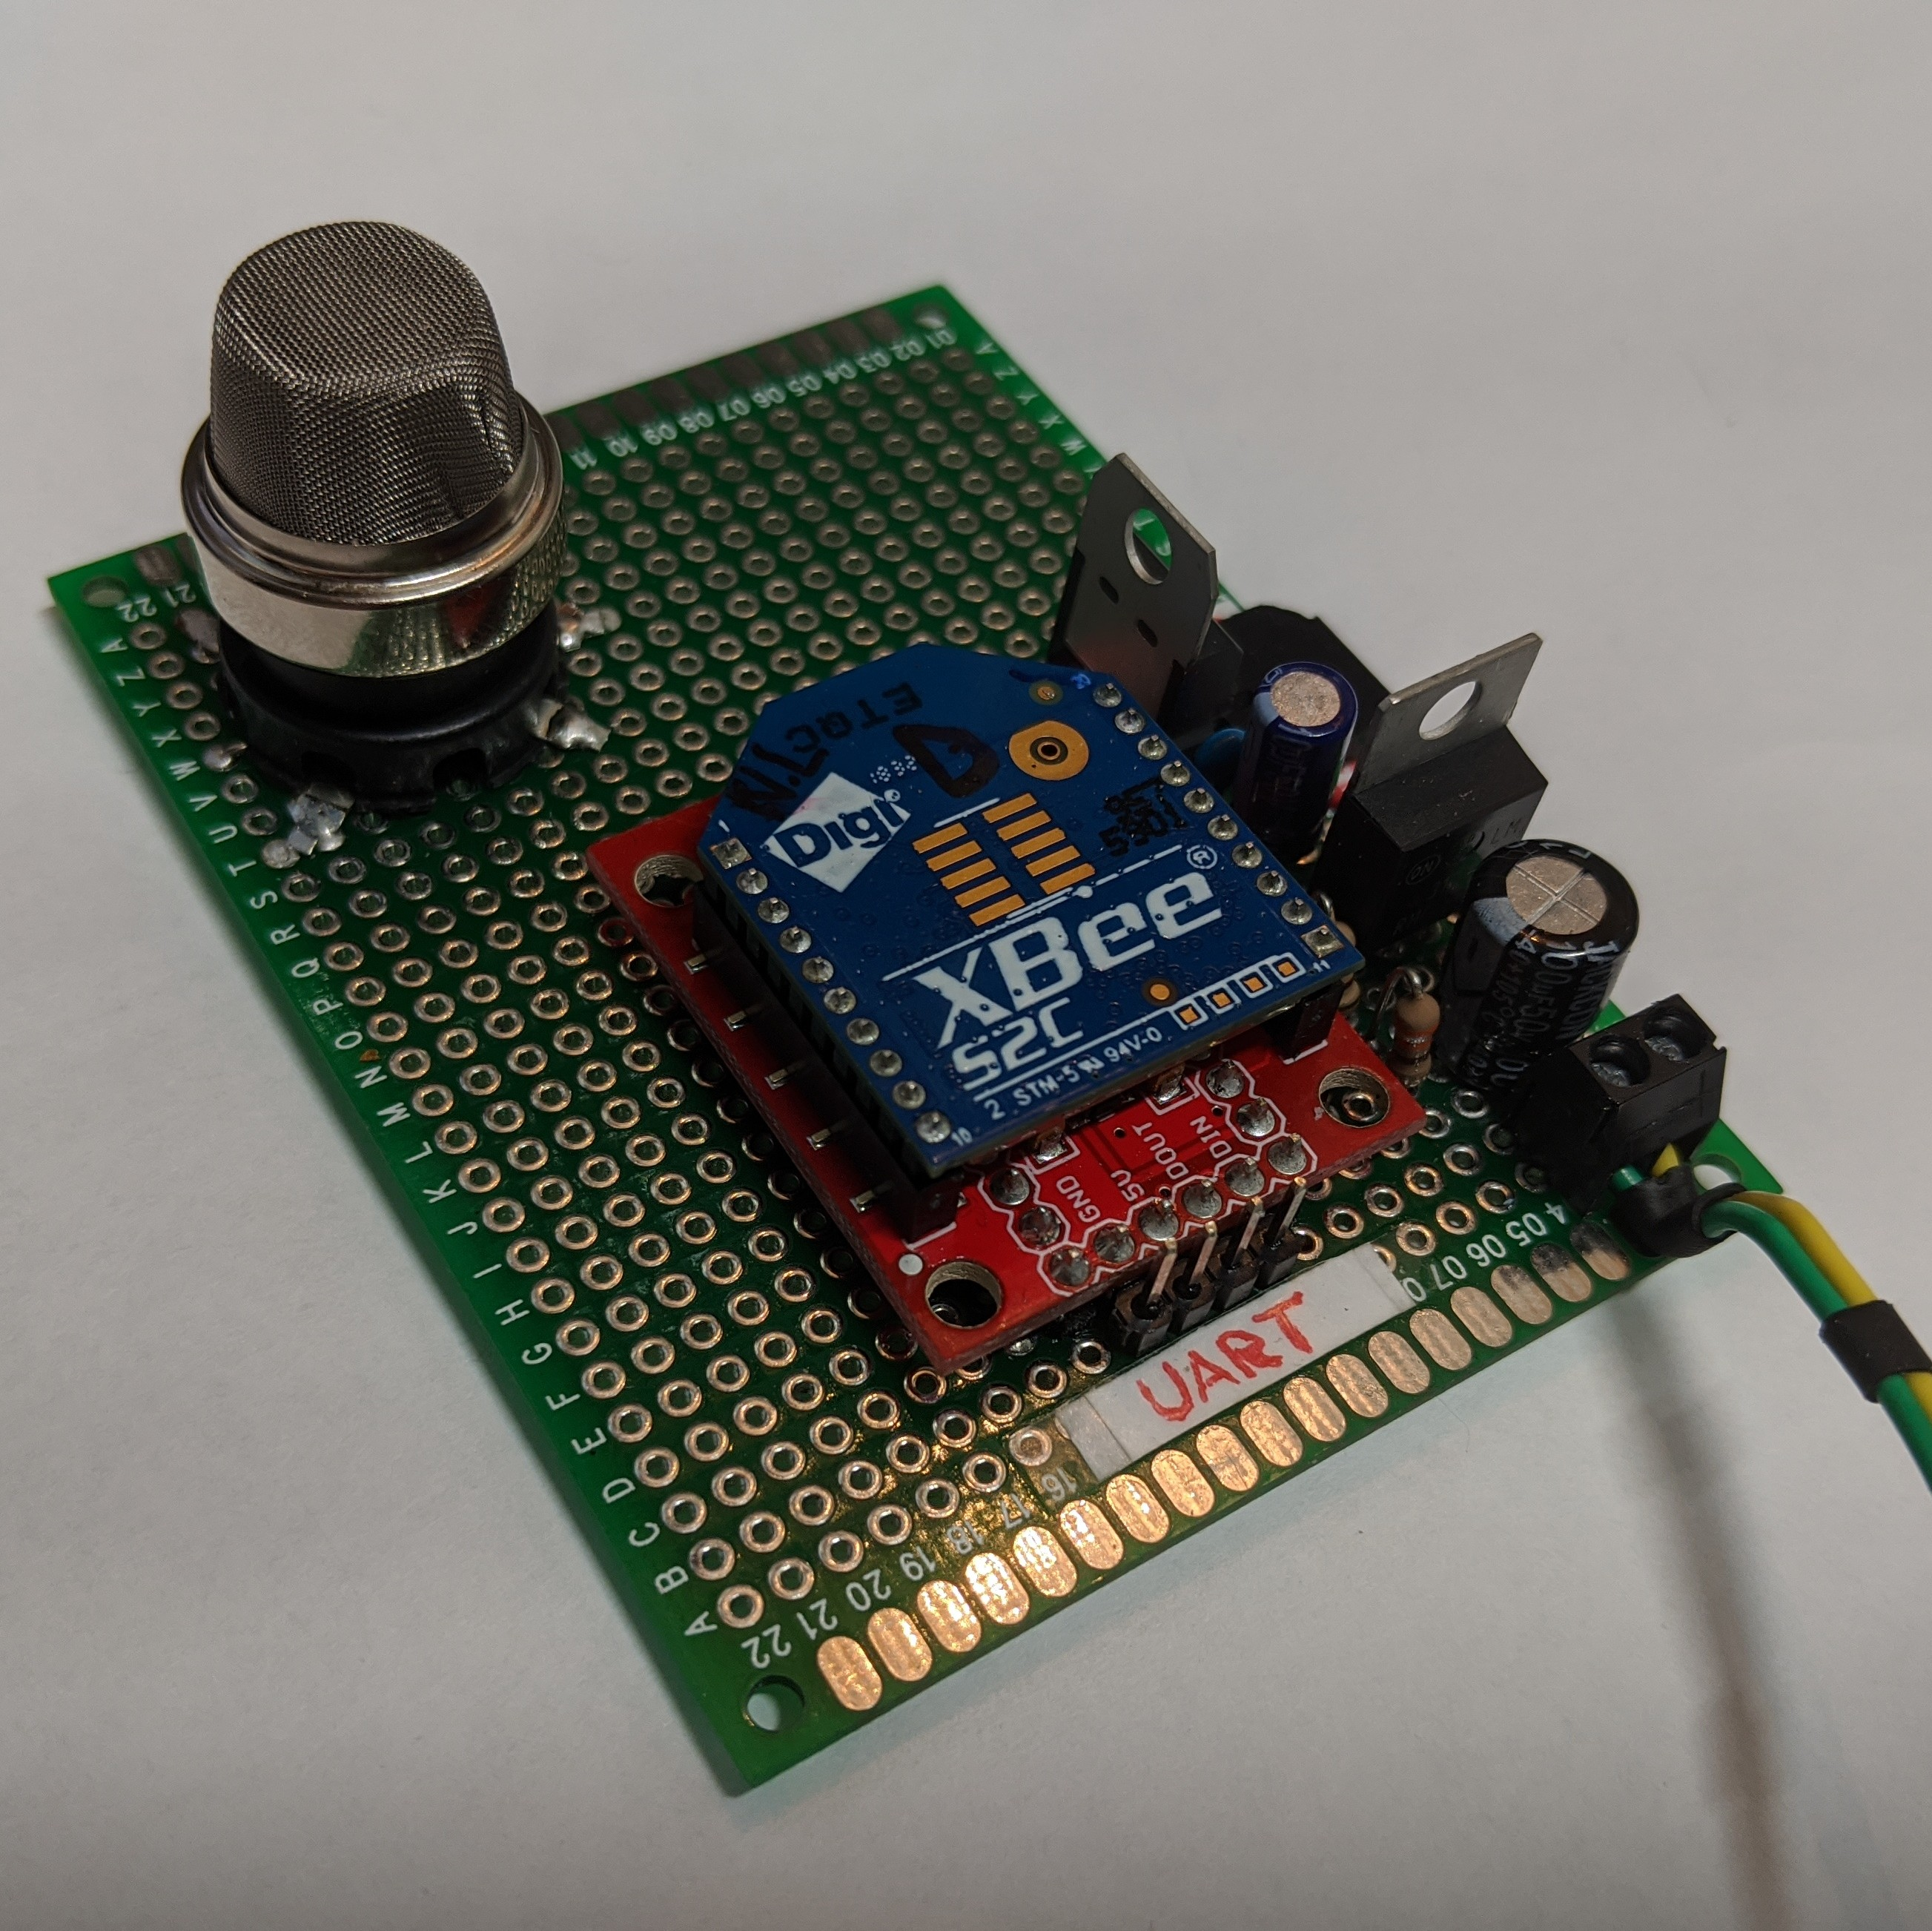
\includegraphics[height=1.5in]{module_gas.jpg}
			\caption{Gas Module}
		\end{subfigure}
		\begin{subfigure}[t]{0.45\textwidth}
			\centering
			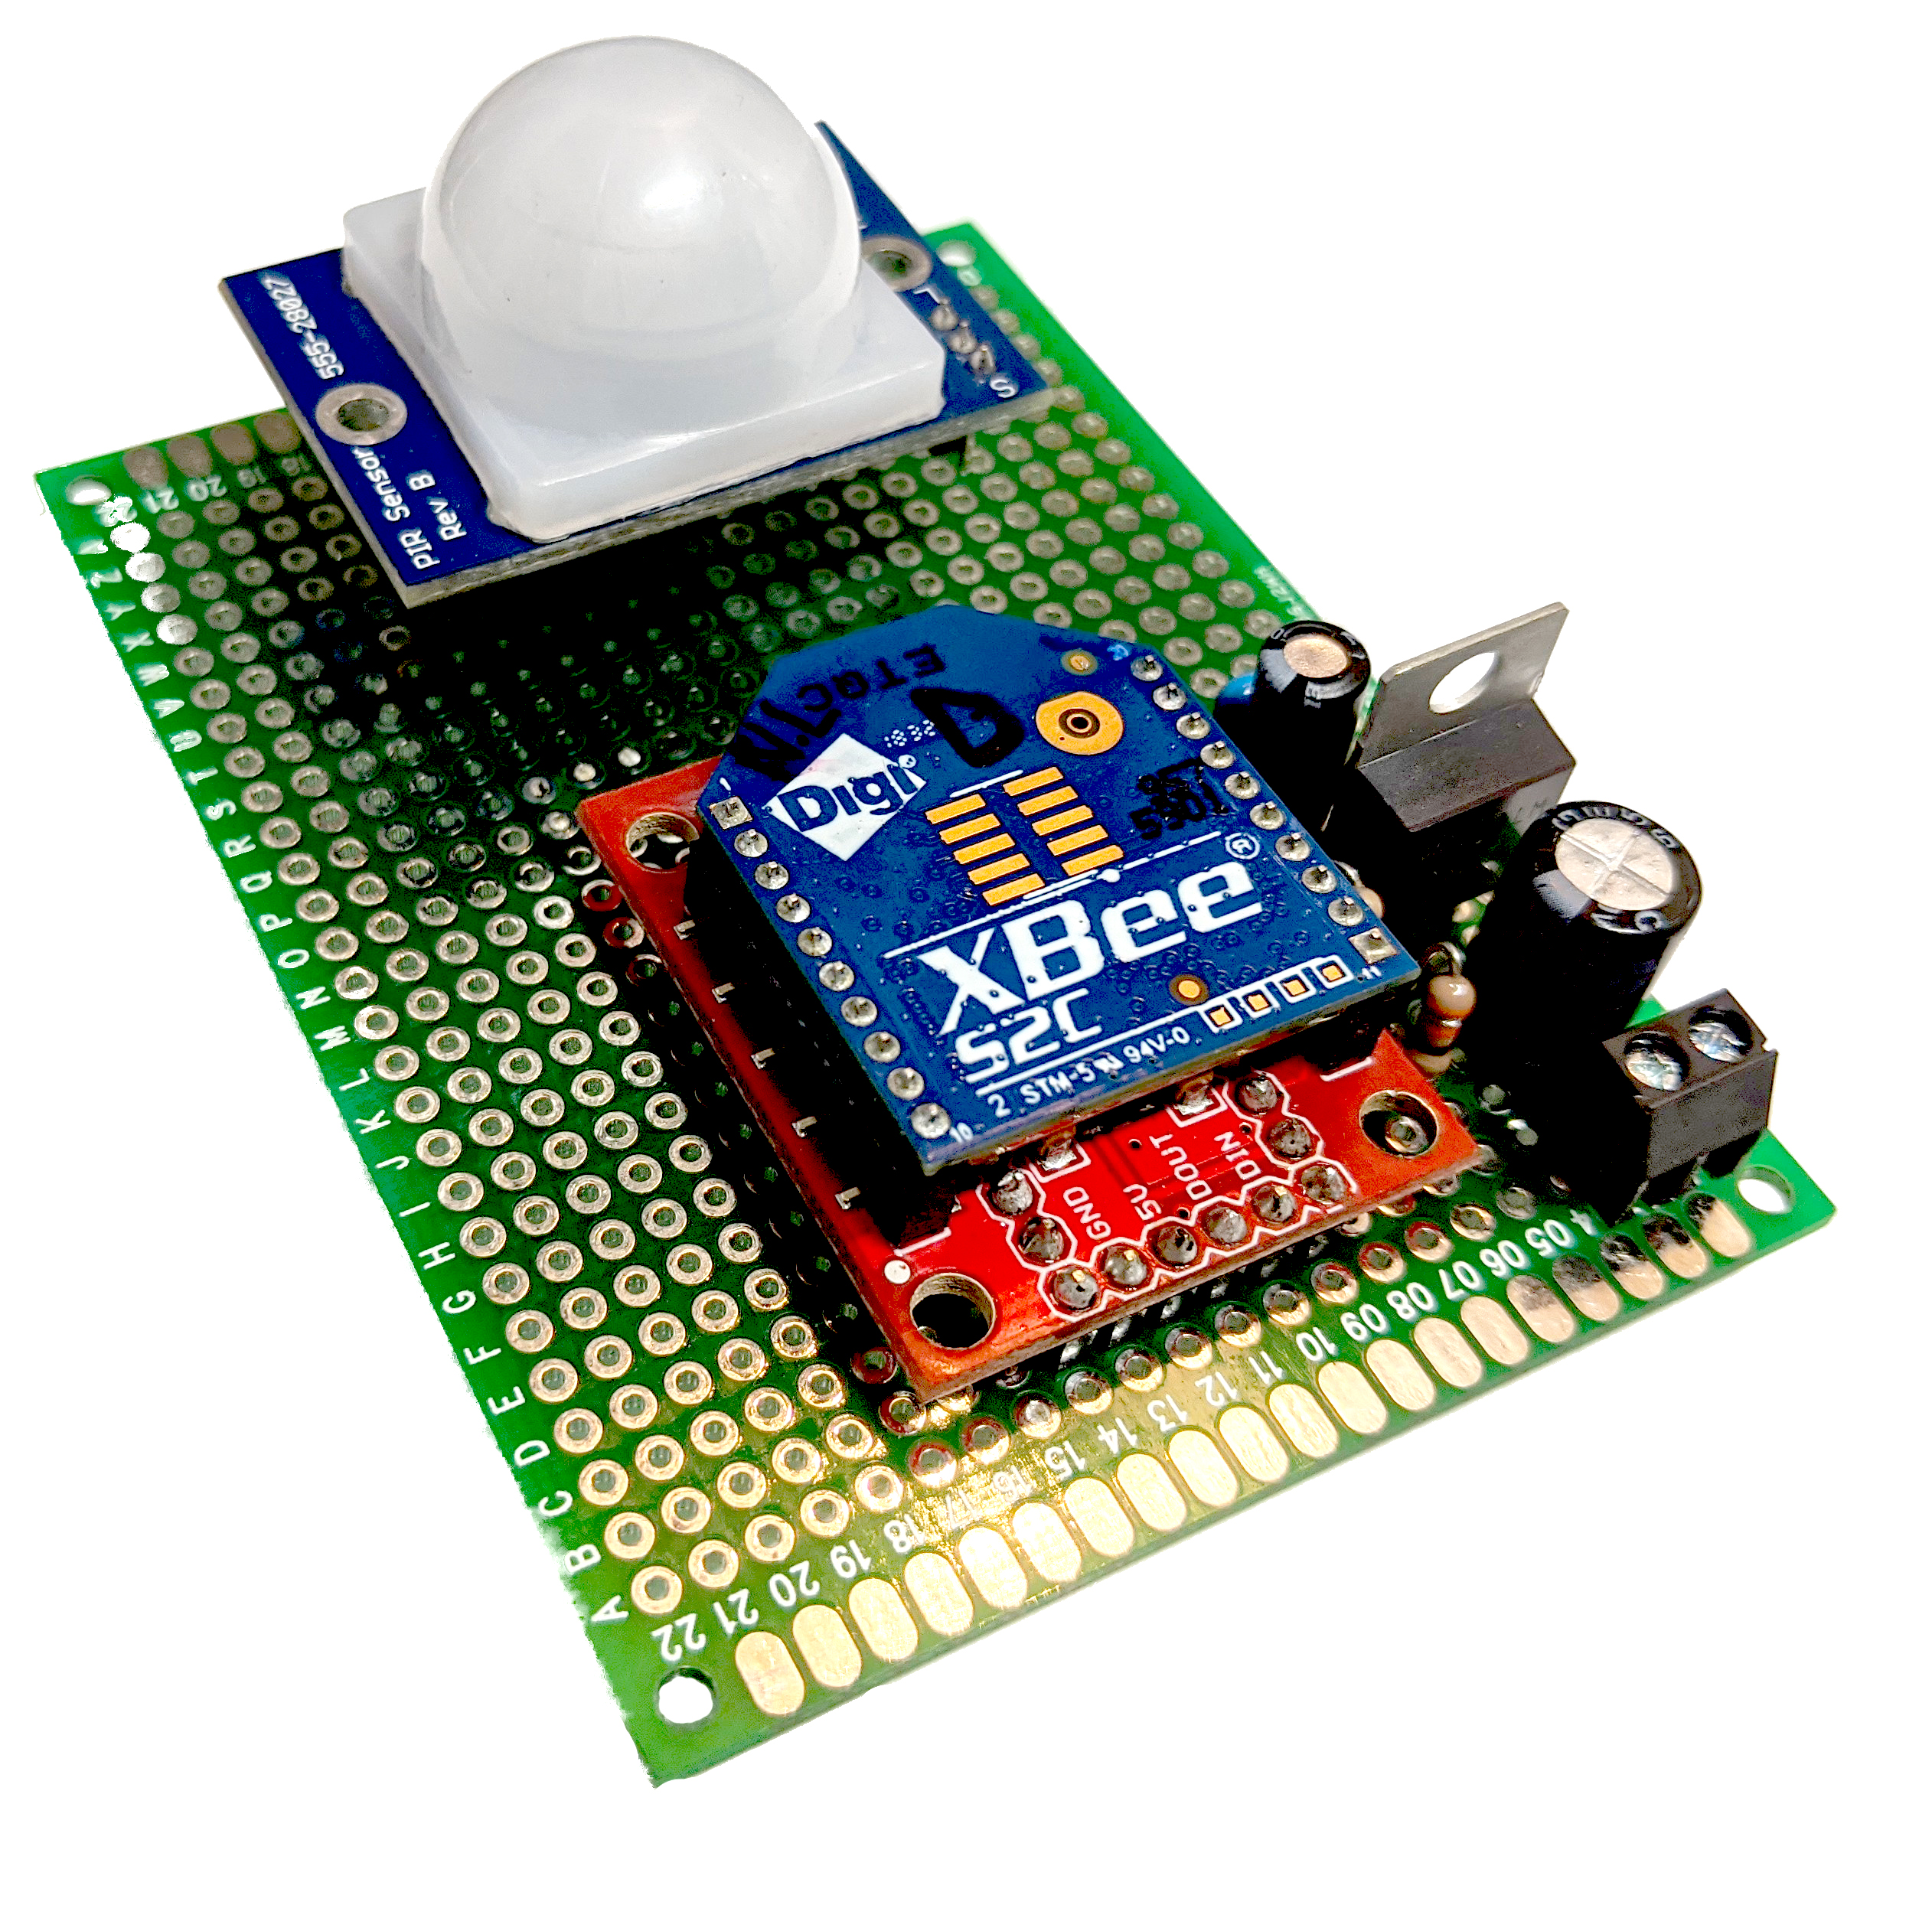
\includegraphics[height=1.5in]{module_motion.jpg}
			\caption{Motion Module}
		\end{subfigure}
		\caption{Internals of Gas (a), and Motion (b) sensing units}
	\end{figure}
	\par The gas sensor module requires two power supplies, one 3.3 volts to power the XBee itself and 5 volts to operate the Tin Dioxide (SnO2) gas sensor. \\
	\par Our system consists of 4 separate modules:
	\begin{itemize}
		\item Coordinator Module - Connects directly to the PC, connects to user interface and controls messages between subsequent end point modules. 
		\item LP Gas Module - A liquid petroleum gas sensor to detect gas leaks in the home. Can detect a wide range of flammable gasses commonly found a typical home.
		\item Motion Sensing Module - The motion sensing module will detect movement and trigger a system response to suit. The Motion module is stand alone to allow the as much freedom of placement as possible.
		\item Door Camera/Lock Module - This module, when directed to do so, can take an image of the area as well as lock the door automatically. This is the most complicated module in the system and includes a Raspberry Pi to transfer frames over the local area network.
	\end{itemize}